\documentclass[10pt, a4paper]{article}

\usepackage{graphicx}
\usepackage{changepage}
\usepackage[rightcaption]{sidecap}

\title{Rapport bibliographique : Modélisation et fabrication d’un actionneur pneumatique souple}
\author{Loïc Mosser, Master IRIV, Parcours IRMC}
\date{Avril 2020}

\begin{document}

\makeatletter

    \begin{titlepage}
    
        \begin{center}
             
            \begin{figure}[!htb]
            \begin{adjustwidth}{-3cm}{-3cm}  
               \begin{minipage}{0.30\textwidth}
                 \centering
                 
\includegraphics[width=1\linewidth]{Logo/Icube.png}
                 
               \end{minipage}\hfill
               \begin{minipage}{0.30\textwidth}
                 \centering
                 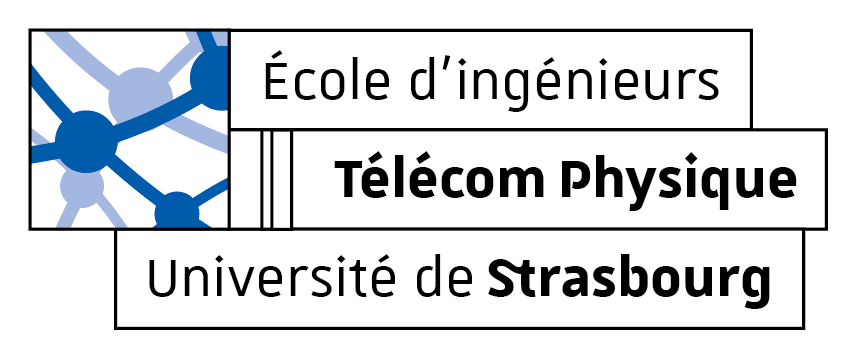
\includegraphics[width=1\linewidth]{Logo/TPS.png}
               \end{minipage}\hfill
               \begin{minipage}{0.30\textwidth}
                 \centering
                 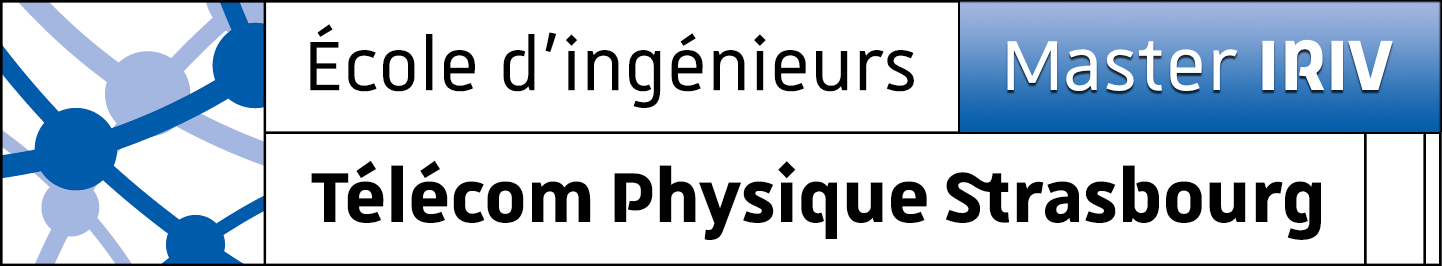
\includegraphics[width=1\linewidth]{Logo/IRIV.png}
               \end{minipage}\hfill
               \begin{minipage}{0.30\textwidth}
                 \centering
                 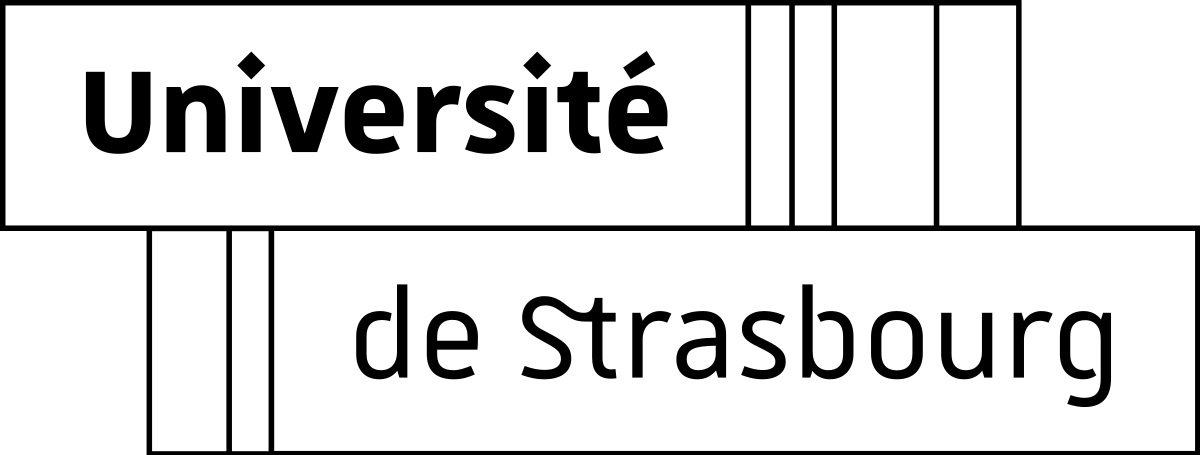
\includegraphics[width=1\linewidth]{Logo/Strasbourg.svg.png}
               \end{minipage}
               \end{adjustwidth}
            \end{figure}
            

            {\huge \bfseries  \@title }\\[15ex] 
            {\LARGE  \@author}\\[10ex] 
            {\large  Encadrants :}\\[2ex] 
            {\large  Pierre Renaud}\\[2ex] 
            {\large  Laurent Barbé}\\[2ex] 
            {\large  François Geiskopf}\\[17ex] 
            
            {\large \@date}
        \end{center}
        
    \end{titlepage}
\makeatother
\thispagestyle{empty}
\newpage

%Add content for page two here (useful for two-sided printing)
%\thispagestyle{empty}
%\newpage
%\maketitle
%\setcounter{page}{1} %Start the actually document on page 1

\tableofcontents
\newpage

\section{Introduction}
    \subsection{Intérêt de l'actionnement linéaire dans le cadre de l'IRM}
    
    \qquad L'Imagerie par Résonance Magnétique (IRM, figure \ref{fig:IRM}) est un dispositif d'imagerie médicale couramment utilisée pour le diagnostique et le suivi de traitement chez des patients atteints de cancers notamment. Elle utilise un champ magnétique fixe de l'ordre du tesla et un champ tournant pour fonctionner.   \\


\begin{figure}[ht!]
\centering
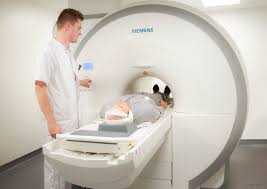
\includegraphics[scale=1]{ImageIntro/IRM.jpg}
\caption{Image d'un dispositif d'IRM avec un opérateur et un patient qui s'apprête à subir un examen (source : http://www.angers-radiologie.fr/examen-radiologique/irm/) }
\label{fig:IRM}
\end{figure}


    Il est possible d'utiliser ce dispositif avec d'autres, comme des stimulateur pneumatiques, pour mesurer des grandeurs secondaires comme le module de cisaillement des tissus mous. C'est le cas de l'élastographie par résonance magnétique par exemple (figure \ref{fig:ERM}).
    
\begin{figure}[ht!]
\centering
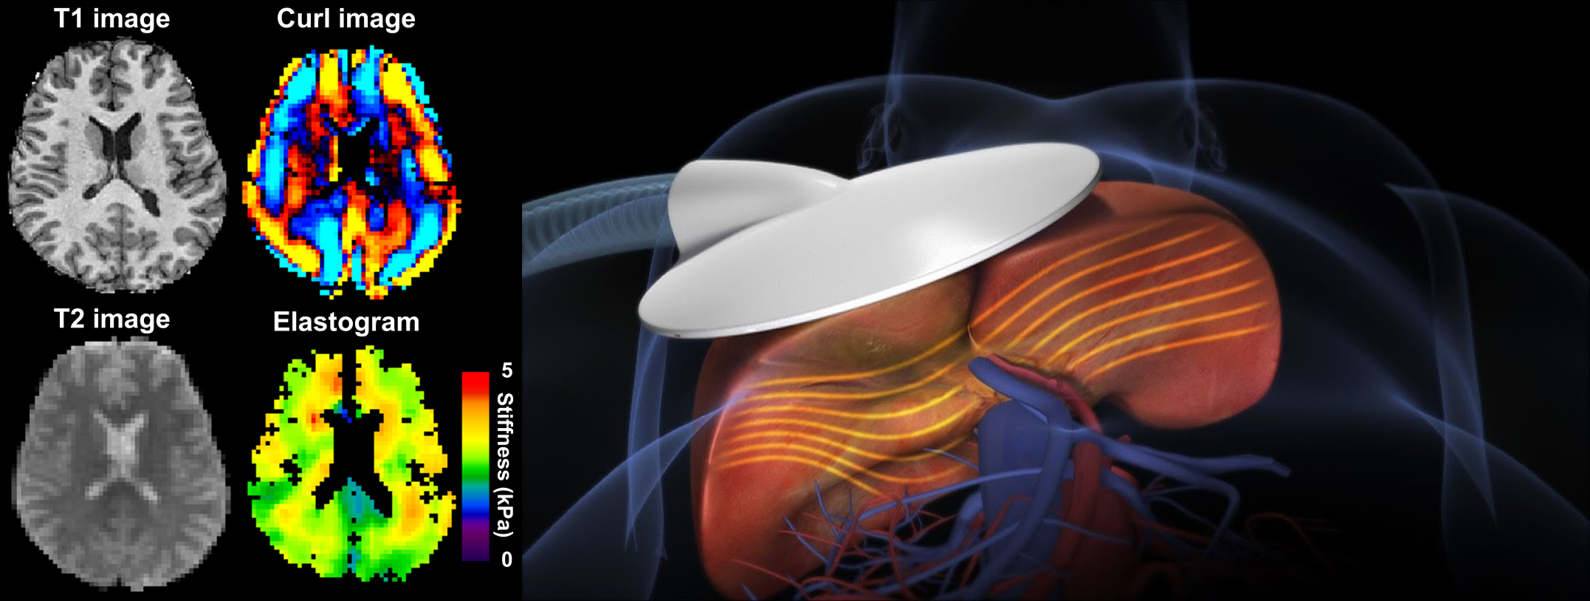
\includegraphics[scale=0.4]{ImageIntro/ERM.png}
\caption{Image du dispositif d'ERM avec son palpeur (à droite) et les image ainsi obtenues (à gauche)}
\label{fig:ERM}
\end{figure}

Il est maintenant possible d'envisager l'utilisation de cette modalité d'imagerie pour guider un geste médical comme l'apport d'un traitement en un point précis du corps du patient. L'insertion d'aiguille, et l'actionnement en milieu IRM plus généralement, devient alors une problématique qui, une fois résolue, permettrai d'assurer un plus haut taux de réussite de thérapie diverses comme ... ce qui entraînerai alors une réduction des coûts associés au traitement des complications dues à une mauvaise manipulation.
    
    \subsection{Problématique associée}
\qquad L'introduction de corps dans le tunnel d'un IRM est une problématique complexe car, au delà du fait que tout corps ferro-magnétique est proscris en IRM, il est nécessaire de s'assurer que le corps introduit n'induise pas d'artefacts de mesure par l'IRM (figure \ref{fig:IRM-Artefact}). En effet, certains matériaux pouvant déformer le champ fixe par leurs présence, la mesure et la reconstruction effectuée dans la traitement ne pourra pas être effectuée correctement. Le système d'aide au geste médical doit donc prévoir cet aspect du milieu dans lequel il évolue. De plus, à cause des éventuelles boucles présentes dans le système, des courants induits peuvent poser des problèmes d'échauffement dans l'appareil d'imagerie.


\begin{figure}[ht!]
\centering
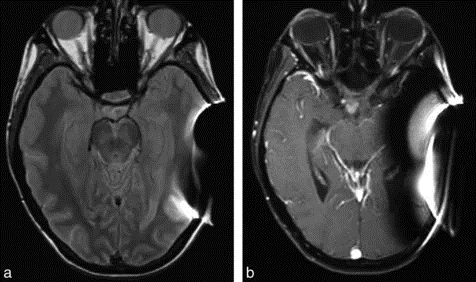
\includegraphics[scale=0.5]{ImageIntro/artefacts.png}
\caption{Artefact dans une image issue d'un IRM causée par un objet métallique (source : https://clemedicine.com/11-artefacts-en-imagerie-par-resonance-magnetique/ ) }
\label{fig:IRM-Artefact}
\end{figure}
    
\section{Système actuel} 

    \subsection{Architecture}
    
\begin{figure}[ht!]
\centering
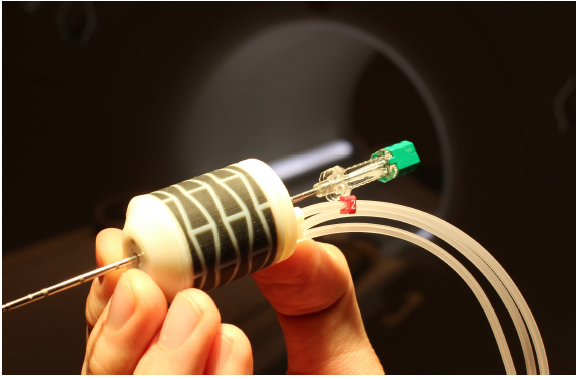
\includegraphics[scale=0.5]{ImageIntro/Inchworm.PNG}
\caption{ Système Actuel (source : Pfeil 2018)}
\label{fig:Inchworm}
\end{figure}   

        \qquad Le système mis en place pour faire de l'actionnement linéaire d'aiguille s'articule autour de celle-ci pour réaliser son actionnement. En effet, le système épouse complètement l'aiguille pour un guidage précis et complet (figure \ref{fig:Inchworm}). Il se décompose en trois parties (figure \ref{fig:planInchworm}): deux mors de serrage et une chambre auxétique. Ces trois parties permettent l'actionnement Inchworm par l'actionneur sur l'aiguille. Ce fonctionnement est décrit partie 3.2.2. Les trois parties sont alimentées en énergie pneumatique de manière indépendantes pour assurer ce fonctionnement. L'énergie pneumatique est une forme d'énergie à privilégier dans le contexte IRM, tout comme l'énergie hydraulique. Nous le verrons par la suite, l'actionnement fluidique est privilégié dans le contexte de l'IRM.
        
\begin{figure}[ht!]
\centering
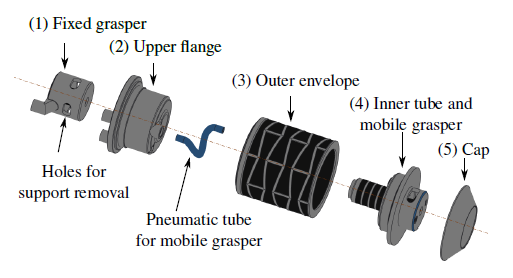
\includegraphics[scale=0.7]{ImageIntro/planInchworm.PNG}
\caption{ Vue éclaté de l'actionneur et des trois parties principales }
\label{fig:planInchworm}
\end{figure}
        
    \subsection{Matériaux et procédé}

        \qquad Actuellement, le système est réalisé par fabrication additive bi-matériaux avec la technologie polyjet (Pfeil 2018) (figure \ref{fig:fabPoly}). La pièce est donc fabriquée à l'aide d'un dépôt de photopolymère dont la polymérisation est réalisée grâce au passage d'une lampe UV. Le dépôt successif de matière permet la polymérisation de la première couche et des couches précédentes. L'utilisation d'un matériau de support facilement traitable permet la fabrication de formes particulière et souvent difficiles à réaliser avec d'autres méthodes. Ce procédé est très adapté aux fabrication de petites séries de pièces et au développement de nouvelles applications. 
        
\begin{figure}[ht!]
\centering
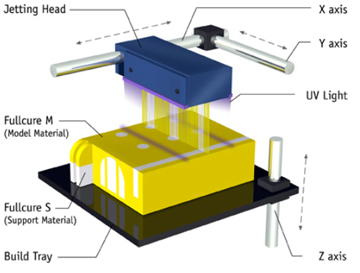
\includegraphics[scale=0.5]{ImageIntro/polyjet_process2.jpg}
\caption{ Illustration du procédé de fabrication utilisé pour réaliser le système original }
\label{fig:fabPoly}
\end{figure}        

    \subsection{Structure auxétique}
        \qquad Une des composantes du système permet l'avance de l'aiguille, c'est la chambre auxétique (figure \ref{fig:maillageAux}). Cette chambre est composée d'un méta matériaux. C'est à dire que, de manière artificielle, il est possible de donner au matériau, qui la constitue, des propriétés, mécaniques ici, particulières. Cette chambre possède un coefficient de poisson négatif ce qui lui permet de s'allonger lorsque qu'une pression est appliquée à l'intérieur de celle-ci. Un matériau avec un coefficient de poisson positif aurait le comportement inverse, la chambre rétrécirait sous l'action de la pression. Cette chambre ce constitue d'un élastomère permettant l'étanchéité et d'une structure rigide possédant un maillage (figure \ref{fig:maillageAux}) qui lui confère ses propriétés particulières.
        
\begin{figure}[ht!]
\centering
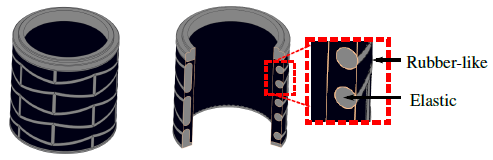
\includegraphics[scale=0.8]{ImageIntro/mailleAux.PNG}
\caption{ Représentation 3D de la chambre auxétique avec le maillage en matériaux rigide et de l'enveloppe en élastomère (source Pfeil 2018) }
\label{fig:maillageAux}
\end{figure} 
        
    \subsection{Préhension}
        \qquad Le maintient de l'aiguille est permis par deux mors (figure \ref{fig:mors}) reliés entre eux par la chambre auxétique. Ces mors peuvent assurer un effort appliqué sur l'aiguille de 5N (rapport d'étude interne) sous une pression de 2 bars. La pression
        
\begin{figure}[ht!]
\centering
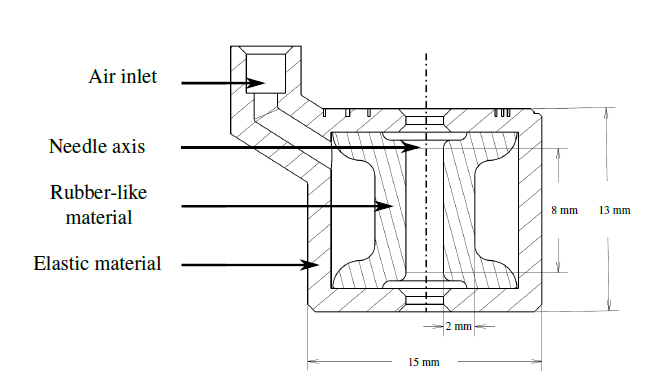
\includegraphics[scale=0.5]{ImageIntro/mors.PNG}
\caption{ Schéma plan d'un mors utilisé dans le système }
\label{fig:mors}
\end{figure} 

\section{Technologie d'actionnement Linéaire dans le cadre de l'IRM}
    \subsection{Type d'actionnement}
        \subsubsection{Actionnement piézoélectrique/ultrasonore}
            Présentation de l'actionnement avec ces technologies. Présentation également des problématiques associés à leur utilisation dans le milieu IRM.
        \subsubsection{Actionnement fluidique}
            Présentation de l'actionnement fluidique dans le cadre de l'IRM avec des système qui l'utilisent déjà.
    \subsection{Génération de mouvement}
        \subsubsection{Transfert de mouvement}
        Caractérisation des cinématiques classiques pour l'actionnement linéaire en IRM
        \subsubsection{Inchworm et systèmes pas à pas}
        Caractérisation du fonctionnement Inchworm

\section{Méta matériaux} 
    \subsection{Structure Auxétique}
    Présentation de la diversité de ces mailles et de leurs cas d'utilisation, la modélisation suit partie suivante
    \subsection{Actionneur renforcés par fibres}

\section{Modélisation et simulation} 
    \subsection{Méthodes de conception des méta matériaux}
        Présentation de la littérature pour la caractérisation des méthodes de conception de structures auxétiques (simulation élément finis, modèle analytique, expérimentations)
    \subsection{Méthodes de validation des caractéristiques des méta matériaux}
        Présentations des méthodes de validations expérimentales employées. Mettre en avant une complexité de fabrication ce qui mène parfois à une absence de fabrication des modèles envisagés. Rebondir avec la partie suivante
        
\section{Matériaux et procédés} 
    \subsection{Fabrication additive par photo-polymérisation}
    \qquad Comme décrit dans la partie 2.2 précédente, le procédé de fabrication par dépôt de photopolymère permet de réaliser des pièces en petites séries et de créer des géométries que les autres procédés ne peuvent réaliser. Néanmoins, ce procédé a des limites. En effet, les matériaux mis en formes n'ont pas les propriétés du matériaux initialement utilisé. Le procédé dégrade celle-ci. La communauté scientifique s'accorde sur le fait que beaucoup de paramètres influe sur les propriétés mécaniques des pièces formées. La position dans le plan de travail (Barclift 2012, Gay 2015), l'orientation de fabrication (Beltran 2015, Gay 2015), la densité et le motif de remplissage (Barnik 2018,Yang 2019). \newline\newline
    
    \quad  Parmi les propriétés altérées apr le procédé de fabrication, on retrouve le module d'Young qui, en plus de diminuer globalement, devient anisotrope à cause de la fabrication couche par couche dans une direction donnée. Néanmoins, dans le cadre de la photo-polymérisation, il est envisageable de considérer ce phénomène comme secondaire dans la mesure où l'on dépose une couche de photo-polymère sur une couche qui n'est pas complètement polymérisée. Alors,le tout forme un ensemble relativement homogène (Barclift 2012). Néanmoins, la résistance à la fatigue et à la rupture sont grandement impactés par le procédé car chaque couche est une potentielle amorce de rupture (figure ) (Barnik 2019). \\
    
   \quad De plus,le fait que le procédé mette en forme les deux matériaux dans la même étape fait apparaître des problèmes d'interfaces entre ceux-ci. Une interface entre ces deux matériaux devient alors une amorce de rupture potentielle supplémentaire ce qui réduit la résistance de la pièce à la fatigue et à la rupture (figure \ref{fig:essai}) (Moore 2015, Vu 2015). 
    
\begin{figure}[ht!]
\centering
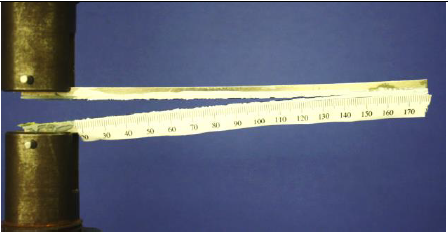
\includegraphics[scale=1]{ImageIntro/EssaiInterfaceTBVW.PNG}
\caption{ Essai réalisé pour étudié l'interface en les deux matériaux TangoBlack et VeroWhite }
\label{fig:essai}
\end{figure}
    
    \subsection{Surmoulage et usinage}
        \subsubsection{moulage avec noyau}
            présentation du procédé et des limitations que cela entraîne

        \subsubsection{moulage par centrifugation}
            présentation du procédé et des limitations que cela entraîne

        
\section{Conclusion}

\bibliography{Biblio.bib}{}
\bibliographystyle{ieeetr}

\listoffigures

\end{document}